\section{Explicit Typing}
\label{sec:Explicit}
%%%%%%%%%%%%%%%%%%%%%%%%%%%%%%%%%%%%%%%%%%%%%%%%%%%%%%%%
\begin{figure}[h!]
\begin{center}
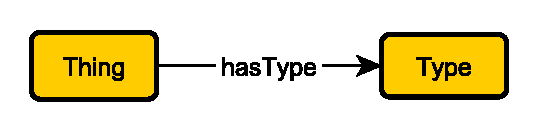
\includegraphics[width=.7\textwidth]{figures/explicit}
\end{center}
\caption{Schema Diagram for the Explicit Typing Pattern. The visual notation is explained in Chapter \ref{chap:prelims}.}
\label{fig:Explicit}
\end{figure}
\subsection{Summary}
\label{sum:Explicit}
%%%%%%%%%%%%%%%%%%%%%%%%%%%%
The pattern for explicit typing is very straightforward. Indeed, it is merely a representation of what we consider to be a "best practice." This pattern is used when there is a finite, but mutable number of types of a thing. We find this easier to maintain than a series of subclass relationships.

%%%%%%%%%%%%%%%%%%%%%%%%%%%%%%%%%%%%%%%%%%%%%%%%%%%%%%%%
\subsection{Axiomatization}
\label{axs:Explicit}
%%%%%%%%%%%%%%%%%%%%%%%%%%%%
\begin{align}
\top &\sqsubseteq \forall\textsf{hasType.Type}  
\end{align}

%%%%%%%%%%%%%%%%%%%%%%%%%%%%%%%%%%%%%%%%%%%%%%%%%%%%%%%%
\subsection{Explanations}
\label{exp:Explicit}
%%%%%%%%%%%%%%%%%%%%%%%%%%%%
\begin{enumerate}
\item Range: the range of \textsf{hasType} is \textsf{Type}.
\end{enumerate}

%%%%%%%%%%%%%%%%%%%%%%%%%%%%%%%%%%%%%%%%%%%%%%%%%%%%%%%%
\subsection{Competency Questions}
\label{cqs:Explicit}
%%%%%%%%%%%%%%%%%%%%%%%%%%%%
\begin{enumerate}[CQ1.]
\item What is the type of Event?
\item Which type of apparatus is that?
\end{enumerate}

\newpage
%%%%%%%%%%%%%%%%%%%%%%%%%%%%%%%%%%%%%%%%%%%%%%%%%%%%%%%%
% End Section
%%%%%%%%%%%%%%%%%%%%%%%%%%%%%%%%%%%%%%%%%%%%%%%%%%%%%%%%
%%%%%%%%%%%%%%%%%%%%%%%%%%%%%%%%%%%%%%%%%%%%%%%%%%%%%%%%